\section{Some definitions}
\noindent
\textbf{Definition} (Helen Gill, 2006) "Cyber-Physical systems are physical, biological, and engineered systems whose operations are integrated, \textbf{monitored, and/or controlled} by a \textbf{computational core}. Components are \textbf{networked} at every scale. Computing is deeply embedded into every physical component, possibly even into materials. The computational core is an embedded system, usually demands real-time response, and is most often distributed"\\

\noindent Roughly speaking a CPS is a \textbf{collection of devices} that:
\begin{enumerate}
    \setlength\itemsep{-.5em}
    \item compute
    \item inter-communicate
    \item interact with the physical word
\end{enumerate}

\begin{figure}[h]
    \centering
     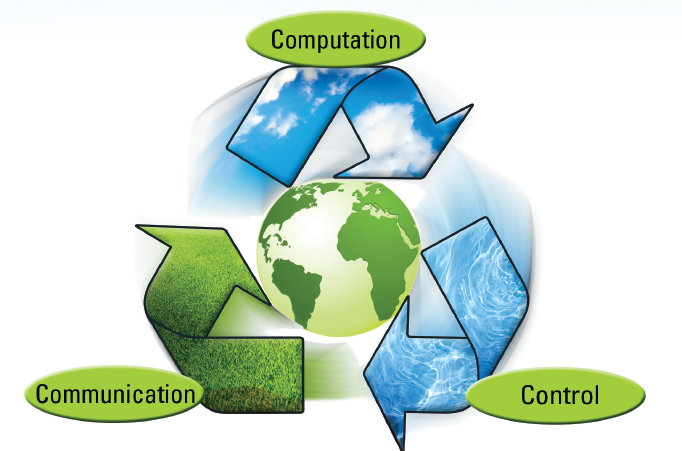
\includegraphics[width=0.6\textwidth]{images/CPS.png}
    \caption{Three Dimensions of CPSs}
    \label{fig:enter-label}
    \end{figure}
    
\noindent 
At this point, we can distinguish in this scenario two layers for CPS: (1) The \textbf{Cyber Layer} which is linked to the computation and communication issues, (2) the \textbf{Physical Layer} deals with the interaction of the devices with the physical word.\\
\vspace{2cm}
%-------------------------------------------------------------

\section{Some examples of CPS}
\noindent
Examples of Cyber-Physical systems could be:
\begin{itemize}
    \item \textbf{Automotive vehicles}: in a car you can find hundreds of sensors, actually we have a computational core, are interconnected in some way (eg. CAN), moreover several feedback-control systems can be find;
    \item \textbf{Teams of mobile robots} that aim to get a target. Robots collaborate to achieve a goal that can be: the exchange of information for example; 
    \item \textbf{Wireless sensor networks} in order to monitor and area (indoor localization without a GPS)
\end{itemize}

%-------------------------------------------------------------
\section{Enabling Technologies and related problems}
\noindent
We can wonder: "How can we deploy CPS?". The answer is by using: 
\begin{enumerate}
    \setlength\itemsep{0em}
    \item \textbf{Embedded systems}: hardware and software integrated within mechanical and electrical systems
    \item \textbf{Sensors and Actuators} for monitoring and control purposes
    \item \textbf{Communication Networks} for example Wireless communication
\end{enumerate}
Despite the \textbf{implementation} it's not too much expensis it raises several issue: at first the \textbf{Vulnerability} which is linked to the \textbf{Safety} of the overall system.

%-------------------------------------------------------------
\section{Mathematical models for CPS}
\noindent
We can modelize a Cyber-Physical System by using: 
\begin{itemize}
      \setlength\itemsep{0em}
    \item \textbf{Basic  Models}: continuos-discrete time LTI systems
    \item \textbf{Hybrid models}: they can describe the interaction between devices and the physical layer including both continuous and discrete events; 
    \item \textbf{Systems under adversarial attacks}: a CPS could be attacked in order to manipulate the exchanged information;
    \item \textbf{Multi-agent systems}: networks of intercommunicating \textit{agents} which may collaborate to reach a \textit{common goal}: \textbf{Consensus}.
\end{itemize}
\subsection*{Hybrid systems}
In order to \textbf{model the presence of physical events} that can change the dynamics, we can consider \textbf{hybrid systems}, also known as  \textbf{switched linear systems}. We can describe them by using the following formalism:
\vspace{1cm}
\begin{large}
    \begin{align*}
    &x(k+1)=A_{q_k}x(k)+B_{q_k}u(k)\\
    &y(k)= C_{q_k}x(k)+D_{q_k}u(k) 
\end{align*}
\end{large}

\vspace{3cm}
for $k=0,1,...$
\begin{itemize}
    \setlength\itemsep{0em}
    \item $x(k)$ is the continuous state
    \item $q_k \in \{1, 2, ..., Q\}$ is the discrete state or {\color{red} mode}, if $q_k \neq q_{k+1}$ then at the time $k$, the dynamics changes, there is a \textbf{switch} for the system
    \item The parameters denoted with \textbf{$A_{q_k}, B_{q_k}, C_{q_k}, D_{q_k} $} are associated witch the {\color{red} active submodel}, the parameters are {\color{blue} piecewise constant}. For this reason the hybrid systems could be seen as a particular case of LTI systems.
\end{itemize}
\noindent
Some examples of hybrid systems could be: a bouncing ball,  a robot moving with obstacles (which are items of the physical layer) in a room etc.

\subsection*{Modeling the presence of attacks}
An attack in the framework of CPS can be modeled as an additive term either on the actuator or the (distributed) sensors.
\begin{align*}
    &x(k+1)=Ax(k)+Bu(k)+b(k)\\
    &y(k)=Cx(k)+Du(k)+a(k)
\end{align*}
Where we indicate with: 
\begin{itemize}
    \setlength\itemsep{0em}
    \item $b(k)$ the attacks on the actuators
    \item $a(k)$ the attacks on the sensors
\end{itemize}

\noindent
We focus only on the term $a(k)$ which can alter the dynamics of the system. We can't model the attacks as a \textit{disturbance/noise} as we could face them by using some techniques of the classical control theory (eg. Loop shaping).\\
A "good attack" can't be modeled in a proper way like a disturbance, but fortunately as the sensors are distributed, the attacks can be done only on a subset of them. There are in the common case \textbf{sparse attacks.}
Our reference model to develop the theory is then the following: 
\begin{align*}
    &x(k+1)=Ax(k)+Bu(k)\\
    &y(k)=Cx(k)+Du(k)+{\color{red}a(k)}
\end{align*}


